\section{Introduction}
Nowadays, a huge number of different products are produced worldwide. Thus, people have more options, leading producers to consider increasing their sales. Thus, they tried to determine each individual's personality and advertise the products customized to their personality type. 
Collecting such data is challenging for researchers because many people don't know their personality type. Thus, researchers tried to extract the personality of people from their tweets. There are other problems because they cannot determine people's personalities just by reading a tweet. Therefore, they are dependent on people again to determine their own personality.
With data generation, we hope to overcome these problems. I put my code for this project on my GitHub\footnote{https://github.com/Babakbehkamkia/Natural-Language-Processing}.


% \section{Data}
% tozihe koli darmorede data

\section{Related Datasets}
% data haye ghabli ro bego
% 2 ta mesal bezan
There is a ready dataset for this task on Kaggle (Myers-Briggs Personality Type Dataset\footnote{https://www.kaggle.com/datasets/datasnaek/mbti-type}). This dataset consists of more than 8600 samples. Each row of this dataset presents a person's personality type and his/hers most recent 50 posts. I used this dataset in the generation phase.

\section{Collection}
I used TweeePy and Twitter API to crawl for tweets that contain a personality keyword like "INFJ". I repeated this procedure for all 16 personality types in MBTI and labeled them with the corresponding keyword.

I created a dataframe for each label and saved it in CSV format. These dataframes consist of 5 columns:
\begin{itemize}
    \item author name
    \item author screen\_name
    \item author id
    \item post
    \item author personality type
\end{itemize}

% \subsection{Data Selection}

\section{Cleaning}
In this section, I describe the cleaning methods I have used to make the raw texts of tweets more processable data.
\begin{itemize}
    \item Necessary cleaning: Removing special characters, stop words, and Lemmatizing the words are done in this part of cleaning.
    \item Removing Hashtags
    \item Removing Links: Links do not have a semantic meaning. Thus, their presents will not improve the model.
    \item Removing Usernames: A name by itself doesn't contain any information. Therefore, I remove usernames.
    \item Removing Retweet Sign: All retweets have the string "RT" in their beginning, which is unnecessary. 
    \item Replacing Emojis: In many related works, researchers tend to delete the emojis. However, they contain a lot of information, and even in some cases, they can change the sentence's meaning. In this work, I replaced all emojis with their corresponding text encode by using the demoji\footnote{https://pypi.org/project/demoji/} library in Python.
\end{itemize}

In the end, I saved the cleaned text in a new column named "cleaned\_text" in the same dataframe.

% todo
% some examples

% \section{Annotation}

\section{Generation}
As told earlier, collecting and annotating data for personality detection is a challenging task. Thus, I tried to generate new samples for each personality type by using GPT-3 API. I created a prompt that contains the personality, a predefined topic (e.g. depression), and an example post from Myers-Briggs Personality Type Dataset with the given personality. With this prompt, I generated some posts toward the given topic and labeled them with the corresponding personality type.
Moreover, in some generated samples, the personality type is mentioned directly. Therefore, I used the [PT] token instead of the personality type.

The generated dataset is saved as a CSV file in the "data/raw" directory. Each file has three columns:
\begin{itemize}
    \item generated post
    \item topic of the post
    \item personality type
\end{itemize}


% todo
% some samples

\section{Statistics}

I used nltk library for the following:
\begin{itemize}
    \item \textbf{nltk.tokenize.TweetTokenizer}: tokenizing the words
    \item \textbf{nltk.corpus.stopwords}: removing stopwords
    \item \textbf{nltk.stem.WordNetLemmatizer}: Lemmatizing the words
    \item \textbf{nltk.word\_tokenize}: breaking samples to words
    \item \textbf{nltk.sent\_tokenize}: breaking samples to sentences
\end{itemize}

\subsection{Basic statistics}

% \begin{adjustbox}{center}
%     \csvautotabular{stats/basic_statistics.csv}
% \end{adjustbox}

% \begin{table}
% \small
% \centering
% \caption{My CSV Table}
% \label{tab:mytable}
% \csvautotabular{stats/basic_statistics.csv}
% \end{table}

\subsubsection{raw data}
\begin{adjustbox}{max width=\textwidth}
\csvautotabular{../stats/basic_statistics_raw_data.csv}
\end{adjustbox}

\subsubsection{clean data}
\begin{adjustbox}{max width=\textwidth}
\csvautotabular{../stats/basic_statistics.csv}
\end{adjustbox}


\subsection{Number of unique common words}

\begin{adjustbox}{max width=\textwidth}
\csvautotabular{../stats/number_of_common_words.csv}
\end{adjustbox}

% \begin{table}
% \small
% \centering
% \caption{My CSV Table}
% \label{tab:mytable}
% \csvautotabular{stats/number_of_common_words.csv}
% \end{table}

% \begin{table}
% \tiny

% \caption{My CSV Table}
% \label{tab:mytable}
% \csvautotabular{stats/number_of_uncommon_words.csv}
% \end{table}
\subsection{Number of uncommon unique words}

\begin{adjustbox}{max width=\textwidth}
\csvautotabular{../stats/number_of_uncommon_words.csv}
\end{adjustbox}

\subsection{Most frequent uncommon words}

According to the number of labels (16), I can only show part of the table in this section. There is a total of 120 (choosing 2 out of 16) possible combinations for the rows of this table.
\newline


\\


\begin{adjustbox}{max width=\textwidth}
\csvautotabular{../stats/most_frequent_uncommon.csv}
\end{adjustbox}

\subsection{Reletive Normalized Frequency}

Due to the same problems as the above section, I only show the first 20 rows of this table.
\newline

\\

\begin{adjustbox}{max width=\textwidth}
\csvautotabular{../stats/RNF.csv}
\end{adjustbox}

\subsection{TF\_IDF}

I used \textbf{TfidfVectorizer} from \textbf{sklearn} in order to compute TF\_IDF.
\newline


\\

\begin{adjustbox}{max width=\textwidth}
\csvautotabular{../stats/tf-idf.csv}
\end{adjustbox}

\subsection{Most appeared unique words}


\end{figure}
\begin{figure}[H]
    \begin{center}
        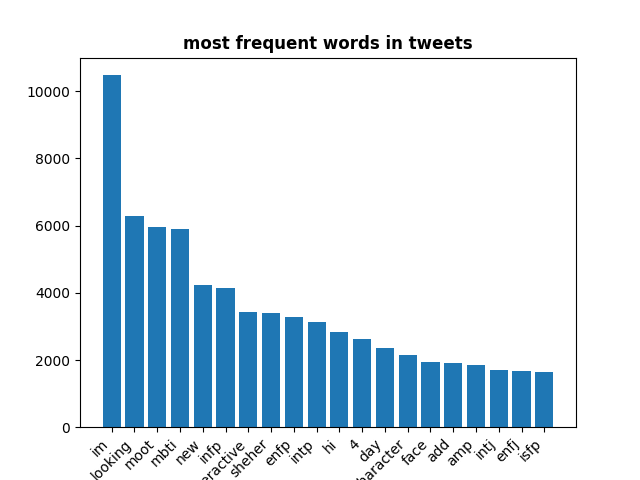
\includegraphics[width=\linewidth]{../stats/frequency.png}
        \caption{most Frequent Words}
    \end{center}
\end{figure}

\section{Scripts}
For this work, bash and batch scripts are provided to run each part or the entire project. The necessary instructions are inside those files.